%===================================
%===================================
%===================================
\setchapterpreamble[u]{\margintoc}
\chapter{Automation overview: modelling, optimization and control}
\labch{intro:automation}

Automation, and particularly process automation, is a multidisciplinary
technology that by integrating various fields of knowledge, aims to develop
autonomous systems, capable of operating with minimal human intervention, using
resources efficiently, adapting to changing conditions, and ensuring safety
and reliability. 

This chapter provides an overview of the main aspects of automation, focusing on
modelling, optimization and control. These three pillars are essential for the
development of advanced automation systems and are widely used in the industry.
The chapter is structured as follows: first, an overview of modelling techniques
is presented, including first-principles and data-driven approaches. Then,
optimization methods are discussed, covering both single-objective and
multi-objective optimization. Finally, control strategies are reviewed, with a
focus on PID control and hierarchical control.

\begin{kaobox}[title=Dealing with complexity]
    Real systems are complex, with many elements interconnected. We first need
    to simplify them into simpler blocks  or levels of abstraction that we can
    work with. These blocks or boxes have inputs and outputs, internally they
    hide some complexity, but from our abstraction we only care that we give
    some input to them, they perform some transformation, and then they return
    some output. These then can be interconnected to form a complex network or
    structure representing the real process. \\
    
    This layering is common in many different fields, for example, processors
    are made up by thousands of layers, with modern processors going from
    city-like structures in the upper layers while reaching atomic scales in the
    lowest layers. \\

    \begin{minipage}{0.4\linewidth}
    \centering
    \includegraphics[width=\linewidth]{figures/microprocessor-min.jpg}\\
    \small Zoomed-in microprocessor. Source: \href{https://www.reddit.com/r/interestingasfuck/comments/ksz30z/oc_i_took_an_old_intel_d320_cpu_and_torn_it_apart/}{stylishpirate - Reddit}
    \end{minipage}
    \hfill
    \begin{minipage}{0.58\linewidth}
    \centering
    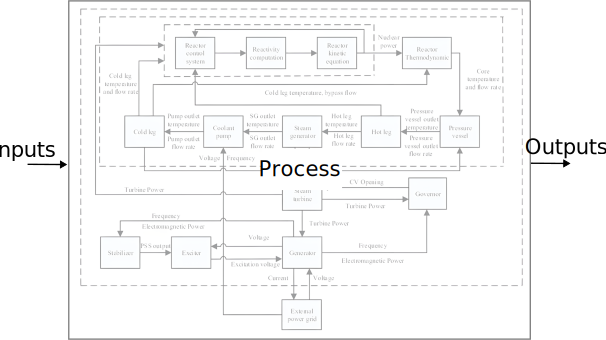
\includegraphics[width=\linewidth]{figures/block-diagram.png}\\
    \small Block diagram with input and outputs
    \end{minipage}
\end{kaobox}

%===================================
%===================================
\section{Modelling and simulation}
\labsec{intro:modelling}

%% Explicación del concepto de modelado %%
Models are  useful  approximations for the real-world
~\sidecite{sokolowski_principles_2011}, more precisely a mathematical
representation of real-world systems. A model can depict a system at different
levels of abstraction depending on the intended use. Models are useful in many
applications: 

\begin{itemize}
    \item Forecasting. They are used to predict the value of a variable at some
    time in the future. 
    \item Simulation. Oftentimes experimentally evaluating real-world systems is
    impractical or infeasible, either because it is costly it may require a lot of
    time, or deteriorate the system among other factors. Simulating a model enables
    the repeated observation of a system with just an associated computational
    cost. 
    \item Control and optimization. in order to compute the optimal input to
    give to a real system, many control strategies are model-based, that is, they
    assess how inputs given to the real system will affect it by first evaluating
    them in a model. 
    \item Analysis of models enables to draw conclusions, verify and validate
    the research, and make recommendations in order to support decision-making.
\end{itemize}

\begin{kaobox}[title=Sensitivity analysis]
    Sensitivity analysis is one of the possible analysis tools. It involves
  systematically assessing how variations in input parameters impact the model
  outputs. > One of the methods used in this research work is the Sobol
  method~\cite{nossent_sobolsensitivity_2011}, which is a variance-based
  approach. This method decomposes the total variance of the model output into
  contributions from individual input parameters and their interactions.
\end{kaobox}

%% Tipos de sistemas: dinámicos, estáticos %%
All real world systems are fundamentally dynamical systems, that is, they
evolve over time. For example a fluid flowing over a plane wing, the spread of a
disease, the climate of a planet, the stock market, planets moving around the
solar system. This behavior takes place continuously with respect to time for
most physical systems, and can be described using differential equations. An
alternative discrete representation can be achieved by performing a
transformation from the continuous space to a discrete space sampling data at
discrete time intervals and is described by difference equations. For an
infinitesimal small time interval they are equivalent. In practice, discrete
representation is a simplification of continuous systems.

An example of the position ($y$) of an object free-falling by gravity could be
represented:
\begin{itemize}
    \item In a dynamic continuous space as $\frac{d^2 y(t)}{dt^2} = -g$
    \item or with a discrete representation (sample time $\Delta t$ and velocity $v$): $y_{k+1} = y_k + v_k \, \Delta t - \tfrac{1}{2} g (\Delta t)^2$
\end{itemize}

\begin{figure}
    \includegraphics[width=\textwidth]{figures/steady-state-transient-concept-plot.png}
    \caption{Dynamic response (reaction curve) of a process output to changes in its inputs'}
    \labfig{intro:modelling:dynamic-response}
\end{figure}

When a dynamic system is left unchanged for a sufficiently long period and an
equilibrium is established between its inputs and outputs, it eventually reaches
a stable or steady state. As long as the inputs remain constant, the outputs
will also remain constant. Thermodynamic processes are often analyzed under
these equilibrium conditions, since the main interest is typically the stable
relationship between a given set of inputs and the resulting outputs, rather
than the detailed trajectory of how the system evolves from one state to
another. This approach makes it possible to evaluate the long-term performance
of the system.

In many cases, a dynamic system can be approximated as a steady-state system if
the transitions between equilibrium states are either negligible or irrelevant
to the problem at hand. Such simplifications are appropriate when the system is
expected to operate mostly under stable conditions, and the transient dynamics
do not significantly affect performance. For example, in thermodynamic analyses,
transient behavior is often treated as noise when evaluating efficiency or
energy balances. This is especially valid for systems with fast dynamics—where
transients settle within seconds—and that are only occasionally disturbed,
meaning the system spends most of its time operating near steady state.

%% Limitations of modelling %%
A model can be an incomplete and possibly incorrect representation of the
phenomenon under study. This typically occurs when information about the
phenomenon is lacking or when very complex processes are being modeled—such as
biological systems that change their dynamics over time, or large-scale
stochastic processes like climate, where small errors can propagate
exponentially. All these factors contribute to uncertainty in modeling.
Uncertainty is generally classified as aleatory or
epistemic~\cite{sokolowski_principles_2011}. Aleatory uncertainty arises from
inherent randomness in the system and is typically addressed through
probabilistic or stochastic methods, though in some cases it may be simplified
or ignored. Epistemic uncertainty, on the other hand, stems from incomplete
knowledge, modeling assumptions, or limited data.

%% Model construction %%
Given a real-world scenario, the first step is to identify a problem to model,
make reasonable assumptions about the process and collect data, choose a
modelling approach, test the assumptions, refine the model as necessary and
finally fit the model to data if appropriate. Two main categories of modelling
exist: first-principle and data-driven, explained in the following.


%===================================
%===================================
\subsection{First principle modelling}
\labsec{intro:modelling:first-principle}

First-principle modelling\sidenote{also called white-box modelling or
physics-based modelling} is an approach to representing a system by starting
from the fundamental laws of nature—such as conservation of mass, energy, and
momentum; Newton's laws of motion; thermodynamics; or chemical kinetics. In this
framework, the model equations are derived from established physical, chemical,
or biological principles that govern the system's behavior.

The resulting models typically take the form of differential and algebraic
equations, which describe how system states evolve over time as a
function of inputs and parameters. Such models are valuable because they provide
physical interpretability, can be extrapolated beyond measured operating points,
and allow deeper insight into how design or operating conditions affect
performance. However, they often require detailed process knowledge, accurate
parameter estimation, and can become computationally intensive for complex
systems.

%===================================
%===================================
\subsection{Data-driven modelling}
\labsec{intro:modelling:data-driven}

Data-driven modelling refers to the construction of models that rely primarily
on measured or simulated data, rather than on explicit knowledge of the
underlying physical laws. The central idea is to capture patterns, correlations,
and dependencies in input--output data and use them for prediction, control, or
optimization. Unlike first-principle models, which are built from conservation
laws and mechanistic equations, data-driven models treat the system as a black
box, with little or no prior assumptions about its internal structure.

A large class of data-driven techniques can be framed within supervised
learning, where the model learns a mapping from inputs to outputs based on
labeled training data. Supervised learning methods are commonly divided into
regression and classification problems: classification predicts discrete
categories, while regression focuses on continuous quantities. In this context,
we are interested mainly in regression approaches, since most engineering
systems require the prediction of continuous variables such as temperatures,
pressures, flows, or performance indices.

Data-driven regression models can range from simple, interpretable
structures—such as polynomial regressions—to highly flexible nonlinear machine
learning models such as Gaussian process regression or artificial neural
networks. Each comes with its own trade-offs between accuracy, interpretability,
data requirements, and computational cost. In the following, we discuss some
representative examples of these approaches.

Data-driven approaches are particularly useful when: adequate experimental or
simulated data is available, predictions are needed mainly within the range of
observed data and simplicity and speed are prioritized over detailed physical
interpretability.

\subsubsection{Polynomial models}

Polynomial models of arbitrary order approximate system behavior by
expressing outputs as polynomial functions of the inputs. The degree of the
polynomial determines how flexibly the model can capture nonlinear
relationships: lower-order polynomials give simple trends, while higher-order
ones can represent more complex patterns but risk overfitting and poor
extrapolation outside the training range.

Polynomial regression is one of the most widely used empirical modeling
techniques because it is easy to implement, computationally efficient, and
provides closed-form solutions for the estimated coefficients. Despite its
simplicity, it often delivers sufficiently accurate approximations for
engineering applications.

Use cases include curve fitting, surrogate models for optimization problems,
quick approximations in control design, and empirical correlations. 

%================================
\subsubsection{Gaussian Process Regression}
\labsec{intro:modelling:gpr}

\todo{Esta sección está por hacer}

%================================
\subsubsection{Artificial Neural networks}
\labsec{intro:modelling:ann}

\glspl[format=long]{annLabel}, as the name suggests, have a behavior similar to
biological neurons. Their structure is formed by a succession of layers, each
one composed by nodes (or neurons) and they receive as input the output of the
previous layer. This process is subsequently repeated until the final layer
which has a number of neurons equal to the number of outputs.

There are important aspects to be considered in the \gls{annLabel} model
design, such as the model configuration, the network architecture and the
network topology. They are discussed below.

% Configuraciones de modelo
\textbf{Model configuration}. If the model has more than one output, several
configurations are available for the implementation of the model as shown in
\reffig{intro:modelling:ann-model-configuration}. The first one is a
\gls{mimoLabel} configuration, where a single network receives all the inputs
and directly produces all predicted outputs. The second one is a cascade
structure. This cascading approach involves training a network (\textit{network
A} in  \reffig{intro:modelling:ann-model-configuration} (b)) to predict one
output using the available inputs. Subsequently, these inputs, along with the
output from the first-output-predicting network, are fed into a second network
(\textit{network B} in \reffig{intro:modelling:ann-model-configuration} (b))
that is in charge of forecasting the second output. This procedure can be
repeated as many times as desired. A potential advantage of this configuration
is that it may reduce the experimental data requirements to obtain satisfactory
results. A third option is the combination of both configurations, where some
networks may predict several outputs, while others are fed some of these
outputs as subsequently use them as inputs. 

\begin{marginfigure}[-7cm]
    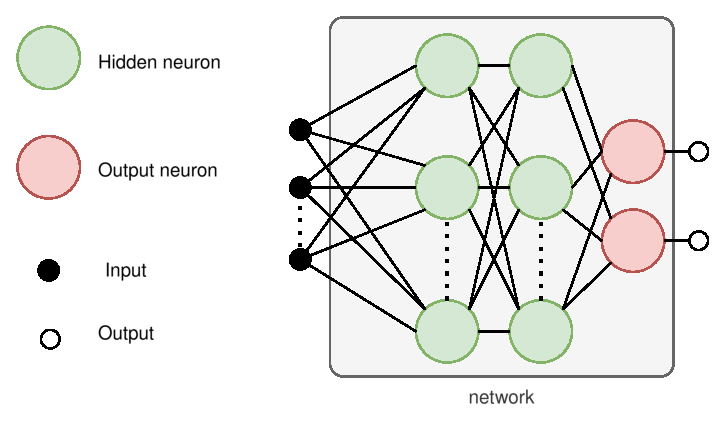
\includegraphics[]{figures/ann_model_configuration_mimo_with_legend.eps}
    {\footnotesize \textbf{(a)} \gls{mimoLabel} configuration\\}
    
    \vspace{1ex}
    
    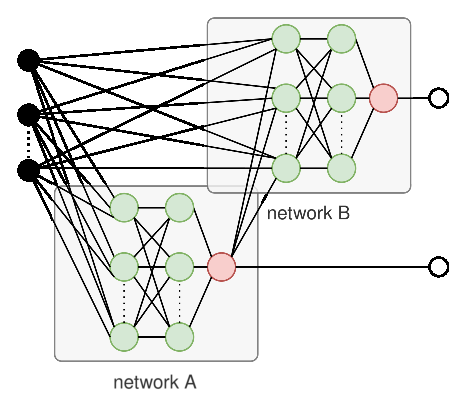
\includegraphics[]{figures/ann_model_configuration_cascade.eps}
    {\footnotesize \textbf{(b)} Cascade configuration}
    
    \caption{\acrshort{annLabel} model configurations}
    \labfig{intro:modelling:ann-model-configuration}
\end{marginfigure}

%As a result, this approach holds the promise of enhanced efficiency in model
%training, potentially requiring fewer data points for accurate predictions. 

% Tipos de red Feedforward Cascade-forward Radial-basis
\textbf{Network architectures}. Three network architectures have been
implemented and tested:
\begin{enumerate}
    \item \gls{ffLabel} network - \reffig{intro:modelling:ann-architectures}
    (a). This is the base network architecture, where different layers are
    added sequentially and the flow of information is unidirectional. The
    transfer function adopted in the hidden layers is the differentiable
    \textit{Log-Sigmoid}\sidenote{Defined as $logsig(x) = 1/(1 + e^{-x})$, mapping any real input to a value between 0 and
    1.}, whereas the one employed in the output layer is a linear one with no saturations.

    \item \gls{cfLabel} network - \reffig{intro:modelling:ann-architectures}
    (b). It is a variation on the feedforward network since it adds direct
    connections from the input and hidden layers to the output layer.

    \item \gls{rbfLabel} network - \reffig{intro:modelling:ann-architectures}
    (c). The transfer functions used in the first layer of the \gls{rbfLabel}
    network are different, they are local Gaussian like functions. Also,
    instead of multiplying by the weights, the distance between inputs and
    weights is computed and the bias is multiplied instead of added
    \sidecite{hagan_neural_2014}.
\end{enumerate}

% \begin{marginfigure}[]
%     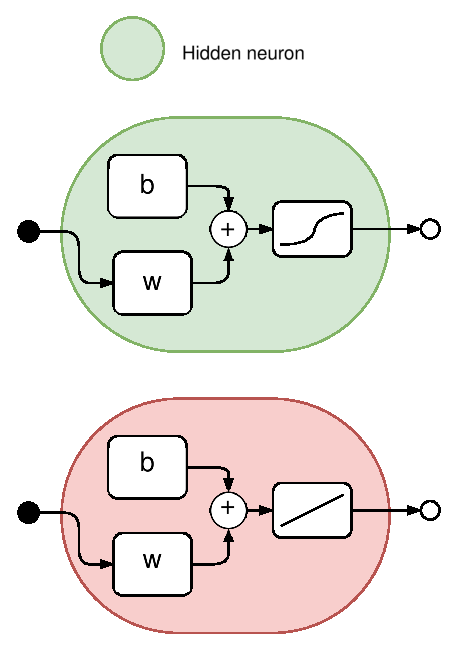
\includegraphics[]{figures/ann_neuron_type_simple_with_partial_legend.eps}
%     {\footnotesize \textbf{(a)} Feedforward\\} \vspace{2ex}
    
%     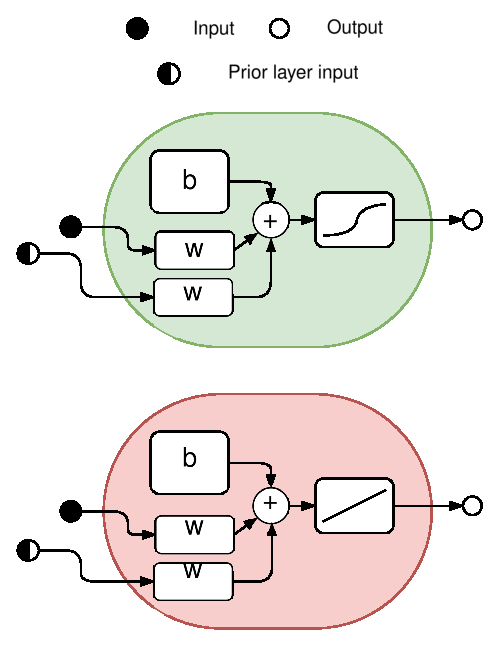
\includegraphics[]{figures/ann_neuron_type_cascade_with_partial_legend.eps}
%     {\footnotesize \textbf{(b)} Cascade-forward\\} \vspace{2ex}

%     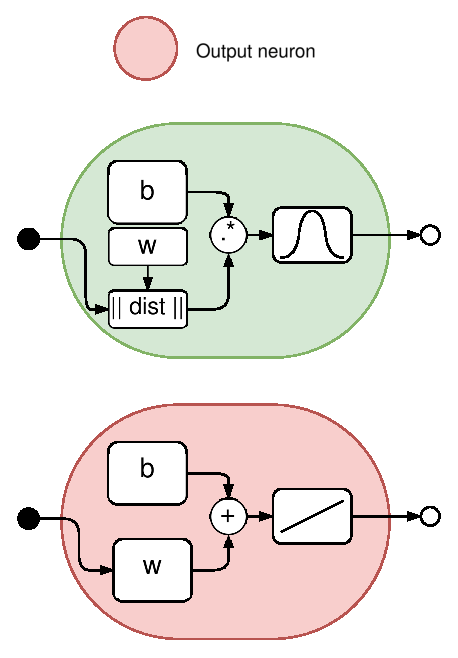
\includegraphics[]{figures/ann_neuron_type_radial_with_partial_legend.eps}
%     {\footnotesize \textbf{(c)} Radial-basis}

%     \caption{Considered \acrshort{annLabel} architectures}
%     \labfig{intro:modelling:ann-architectures}
% \end{marginfigure}

\begin{figure*}[h!]
    \centering
    \subfloat[\centering
    Feedforward]{{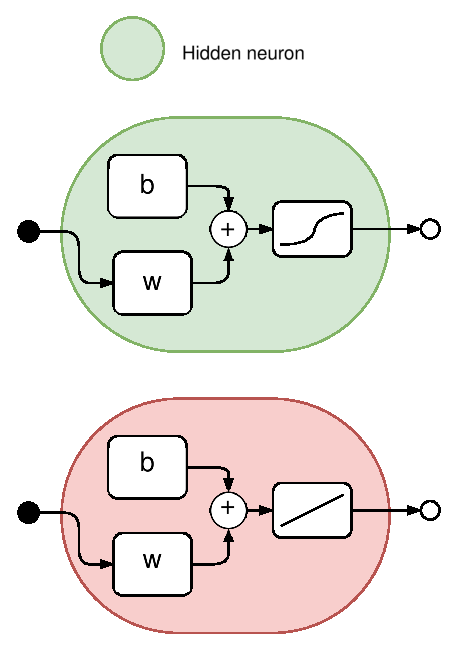
\includegraphics[width=0.32\textwidth]{figures/ann_neuron_type_simple_with_partial_legend.eps}
    }}%
    \qquad
    \subfloat[\centering
    Cascade-forward]{{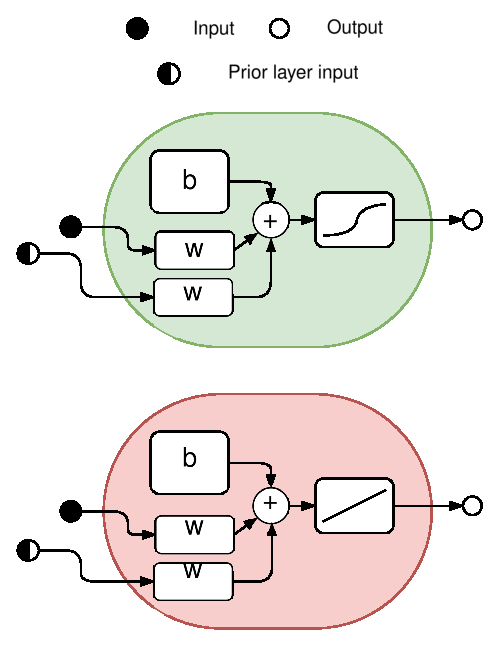
\includegraphics[width=0.32\textwidth]{figures/ann_neuron_type_cascade_with_partial_legend.eps}
    }}%
    \qquad
    \subfloat[\centering
    Radial-basis]{{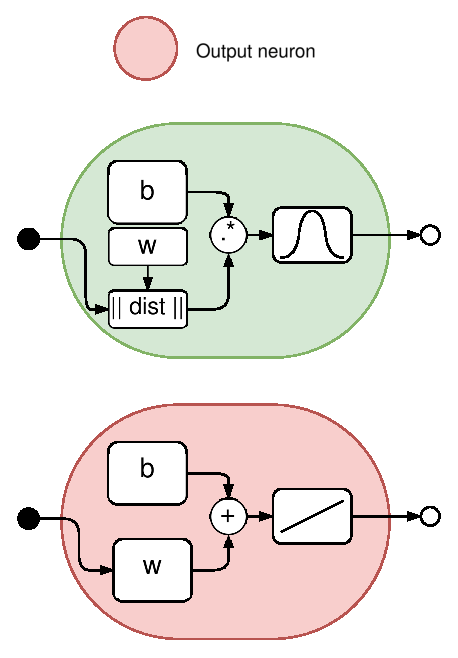
\includegraphics[width=0.32\textwidth]{figures/ann_neuron_type_radial_with_partial_legend.eps}
    }}%
    
    \caption{Considered \acrshort{annLabel} architectures}
    \labfig{intro:modelling:ann-architectures}
\end{figure*}

% topologías de red N de capas N de neuronas por capa

\textbf{Network topology}. Two-layer networks (one hidden and one output layer)
can learn almost any input-output relationship, including non-linear ones.
Adding more layers can improve the learning for more complex problems. However,
increasing the number of layers or neurons per layer increases the training
computational requirements, requires more data for a satisfactory model and can
lead to overfitting. Therefore, the process is usually started with two layers
and then the number of layers is increased if they do not perform
satisfactorily~\cite{hagan_neural_2014}. In this study, for the feedforward and
cascade-forward architectures, one and two hidden layers have been tested with
the following configurations: 5, 10, 20, 5-5, 5-10, 10-5, 10-10. For the case
of the \gls{rbfLabel}, it only has one hidden layer and neurons are added
sequentially during the training process up to a maximum which is set to 120
neurons.

% Procedimiento entrenamiento Justificar mejor elección de algoritmo de
% entrenamiento
\textbf{Training process}. The next important aspect to consider is the
training process. For the \gls{ffLabel} and \gls{cfLabel} networks many
Gradient- or Jacobian-based algorithms can be utilized. In this case, the
Levenberg-Marquardt backpropagation algorithm \sidecite{beale_neural_2010} has
been used. It is a fast algorithm, ideal for multilayer networks with up to a
few hundred weights and biases enabling efficient training. The training in
this case is done in batches since sequential training is slower and does not
produce better results. All data have been normalized applying the z-score
normalization method. 
% Early stop, paciencia For most applications of neural networks, the training
% error never converges to exactly zero. The error can reach zero for the
% perceptron network (radial basis network), but it is unlikely to happen for
% multilayer networks. For this reason, a criteria for deciding when to stop
% the training needs to be set in place, and this criteria needs provide a
% mechanism to avoid overfitting. 
The criteria established for deciding when to stop the training is the
following one:  when the performance on the validation set increases (worsens)
or when the  gradient is below a minimum ($1\times10^{-7}$) for a number of
iterations or epochs, or when a maximum number of 1000 epochs is reached. The
number of iterations to wait, often refereed as patience, is set to 6. Finally,
the selected network parameters will be those of the best epoch.

For each network architecture, the training process was repeated a total of ten
times (this is the recommended practice if the computational requirements allow
it, since it guarantees reaching a global optimum with a high degree of
confidence \sidecite{hamm_comparison_2007}). The optimal architecture and
training was selected according to a performance function, which in this case
has been the \gls{mseLabel} with the values normalized.

In the case of the \gls{rbfLabel} network, the chosen training method consists
in two stages which treats the two layers of the \gls{rbfLabel} network
separately. The first layer weights and biases are tuned based on the
orthogonal least squares method \sidecite{hagan_neural_2014}, while for the
second layer are computed in one step using a linear least-squares algorithm.
During training, neurons are added to the first layer (in increments of 20)
trying to minimize the \gls{mseLabel} to some goal, which in this case is set
depending on the case study: 10 for the \gls{mimoLabel} configuration and 0
($^\circ$C$^2$) and 20 (l$^2$/h$^2$) for temperature and water lost networks,
respectively, for the cascade configuration. Finally, a parameter called spread
is used to set the first layer biases. Larger values of this parameter promote
a smoother approximation of the training data (more generalization),
conversely, lower values provide a more exact fit to the training data. Values
from 0.1 to 30 have been tested for this parameter.


%================================
\subsubsection{Other machine learning methods}

\begin{itemize}
    \item \textbf{Random Forest}. A random forest for regression is a method
    that combines many decision trees to make more accurate and stable
    predictions. A decision tree is a model that splits the data into smaller
    and smaller groups based on input features, creating a set of simple rules
    that lead to a prediction at the end of each branch. Each tree in a random
    forest is trained on a slightly different version of the data by randomly
    sampling both data points and features, and the forest's final prediction is
    obtained by averaging the outputs of all trees. As the number of trees
    increases, the prediction error stabilizes and approaches a fixed value. The
    performance of a random forest depends on how strong the individual trees
    are at predicting the target and how different they are from each other, and
    this balance allows the method to produce reliable predictions that are
    usually better than those of a single decision tree~\sidecite{breiman_random_2001}. 
    
    \item \textbf{Gradient-boosting} builds a strong predictive model by
    combining many weak models, usually decision trees, in a sequential way. Each
    new tree is trained to correct the errors (residuals) made by the previous
    ensemble, using the gradient of a loss function to guide the
    improvements~\sidecite{friedman_greedy_2001}.
\end{itemize}


%===================================
%===================================
\subsubsection{Data-driven from first-principles models. Synthetic dataset generation}
\labsec{intro:modelling:sample-generation}

% Mencionar modelos basados en datos a partir de modelos físicos. Describir
% combinatoria sin detallar la combinatoria particular seguida para el modelo
% del CC.
One important advantage that first-principles models have over data-driven is
their scalability, that is, the ability to adapt a model developed and
validated in a pilot-scale system, to a large scale one. This is true for many
systems as long as the system configuration remains the same. This allows to
study and analyze pilot scale plants and extrapolate the results to industrial
sized plants. In addition, these type of model are also capable of predicting
the behaviour of the modelled systems in conditions that have not been tested
(\eg different operating or environmental conditions), although the
reliability of the model could be lower if these conditions move away from
those experimentally used for some parameter calibration.

On the contrary, data-driven models are very specific to the system and
operating ranges they are trained for. That is why training/calibrating a
data-driven model with data from a first-principles model is a common practice
to obtain a model that can be used in a larger range of operating conditions...

The process of generating samples from a first-principles model to train a
data-driven model is called sample generation. It consists of running the
first-principles model for a set of input parameters, which can be selected
randomly or following a specific distribution, and then using the outputs of
the first-principles model as the training data for the data-driven model.

The first step is to define the input parameters and their ranges. This can be
done by selecting the most relevant parameters for the system and determining
their ranges based on the system's operating conditions. The next step is to
generate a set of input parameters, which can be done using different methods
such as Latin Hypercube Sampling, Monte Carlo Sampling, Sobol Sampling, or
simply grid sampling. These methods allow to generate a set of input parameters
that cover the entire range of the input parameters and ensure that the
generated samples are representative of the system's behaviour. Once the input
parameters are defined, the first-principles model is run for each set of input
parameters, and the outputs of the model are recorded. Finally, the recorded
outputs are used to train the data-driven model.


%===================================
%===================================
\subsection{Discrete modelling by means of \glspl{fsmLabel}}
\labsec{intro:modelling:discrete}

So far we have discussed modelling of continuous systems, where changes evolve
smoothly over time, often described by differential equations. Discrete or
event-driven modelling, on the other hand, focuses on systems where the state
changes only at specific points in time in response to events.

There are many ways of modeling the behavior of these systems, and the use of
state machines is one of the oldest and best known. State machines allow us to
think about the ``state'' of a system at a particular point in time and
characterize the behavior of the system based on that state\sidenote[][*-3]{On each
different state, a process can be governed by different dynamics}.

For example, a traffic light can be described as a finite state machine with
three primary states: \textit{green}, \textit{yellow}, and \textit{red}. In each
state, the traffic light has a well-defined behavior (allowing vehicles to pass,
warning them to slow down, or stopping them completely). The transitions between
states are also clearly defined: green changes to yellow, yellow to red, and red
back to green. Some transitions are possible, while others are not (\eg, green
cannot jump directly to red without first passing through yellow).

\begin{marginfigure}[-3.5cm]
    \centering
    \includegraphics[width=.5\linewidth]{figures/fsm-traffic-light.png}
    \caption{\gls{fsmLabel} representation of a traffic light}
    \labfig{intro:modelling:fsm-traffic-light}
\end{marginfigure}


So, a state machine is a model of behavior composed of a finite number of
\textit{states} and \textit{transitions} between those states. Within each state and
transition some \textit{action} can be performed. A state machine needs to start at
some \textit{initial state}. Finite refers to a machine that has a limited number of
possible states and at any given time it will be in one of those states. Its
core components are described in the following:

\begin{itemize}
    \item \textbf{State}. A state represents a particular condition or stage in
    the state machine. It's a distinct mode of behavior or phase in a process.
    
    \item \textbf{Transition}. This is the process or event that causes the
    state machine to change from one state to another.

    \item \textbf{Action}. Specific operation or task that is performed when a
    certain event happens \ie a state is entered, exited, or during a
    transition.
    
    \item \textbf{Model}. A stateful structure that holds information about the
   state of the machine. It gets updated during transitions and defines
   actions.

    \item \textbf{Machine}. This is the entity that manages and controls the
    model, states, transitions, and actions. It's the conductor that
    orchestrates the entire process of the state machine.
\end{itemize}

\subsection{Forecasting and combinatory nature of \glspl{fsmLabel}}

A traffic light is a simple example of a deterministic state machine, because
its transitions are triggered by a single predictable input — the timer — and
therefore its future trajectory is entirely fixed. From any given state, there
is only one possible next step, so the entire cycle can be anticipated with
certainty (see \reffig{intro:modelling:fsms-evolution} (a)). Many real systems,
however, are not this simple. When the set of inputs that can trigger
transitions is larger and each input leads to different successor states, the
system no longer has just one linear trajectory but many possible ones. In such
cases, the behavior of the machine can be represented as a branching tree, where
each node corresponds to a state and each branch corresponds to a possible input
event. This can be illustrated for the traffic light example if a push-button is
added (see \reffig{intro:modelling:fsms-evolution} (b)). The state will be green
light unless the push-button is triggered. Starting from an initial state,
evaluating now the possible paths that yield in an arbitrary final state given a
number of steps becomes a combinatory problem. 

\begin{figure}
    \centering
    \subfloat[\centering Simple traffic light]{{\includegraphics[width=0.8\textwidth]{figures/fsm-evolution-simple-traffic-ligth.png}}}%
    \vspace{0.1cm}
    \subfloat[\centering Traffic light with push-button]{{\includegraphics[width=0.8\textwidth]{figures/fsm-evolution-traffic-ligth-with-pushbutton.png}}}%
    \caption[Evolution of different traffic-light \glspl{fsmLabel}]{Evolution of different traffic-light \glspl{fsmLabel} assuming the timer takes one step to complete.}
    \labfig{intro:modelling:fsms-evolution}
\end{figure}

This branching has important implications: while the machine is still finite in
the number of states, the number of possible sequences of states over the
horizon grows rapidly as more steps are considered. After just a few
transitions, the tree of possible futures can expand exponentially.

%===================================
%===================================
\subsection{Performance metrics}
\labsec{intro:modelling:metrics}

For models to be useful they need to accurately represent the real process. In
order to quantitatively assess how good a model represents a real system we use
different performance metrics. Four performance metrics are described hereinafter:
coefficient of determination (R$^2$), \gls[format=long]{rmseLabel},
\gls[format=long]{maeLabel} and \gls[format=long]{mapeLabel}. These metrics are
described below.

\textbf{Coefficient of determination}. Regression estimates the relationship
between input variables\sidenote{also known as features} and a continuous output
variable\sidenote{also refereed as target}. R$^2$ is a direct measure of
regression. It measures the proportion of the variance in the predicted variable
that can be attributed to the independent variable(s), in this case the
considered system inputs. Values close to one indicate a better prediction
accuracy. It is calculated as follows:

\begin{equation*}
    R^2 = 1 - \frac{\sum\limits_{i=1}^n (y_i - \hat{y}_i)^2}{\sum\limits_{i=1}^n (y_i - \bar{y})^2},
\end{equation*}

where $y_i$ is the measured or observed value for the output variable, in the
$i-th$ observation, $\hat{y}_i$ is the estimated value of the same variable and
$n$ is the total number of observations. Finally, $\bar{y}$ is the mean value
of the experimental values.


\textbf{Root Mean Square Error}. \gls{rmseLabel} is a statistical measure of
the difference between the values predicted by a model and the observed values.
It is calculated as the square root of the mean of the squared differences
between the predicted and observed values and it has its units. 

% \marginnote{
\begin{equation*}
    \mbox{RMSE} = \sqrt{\frac{1}{n} \sum\limits_{i=1}^n (y_i - \hat{y}_i)^2}
\end{equation*}
% }

\textbf{Mean Absolute Error}. It represents the average absolute difference
between predicted and actual values.

\begin{equation*}
    \mbox{MAE} = \frac{1}{n} \sum\limits_{i=1}^n \left|y_i - \hat{y}_i\right|
\end{equation*}

\textbf{Mean Absolute Percentage Error}. As the \gls{maeLabel}, it calculates
the difference between the predicted and the actual values, but in this case it
does so in relative terms:

\begin{equation*}
    \mbox{MAPE} = \frac{1}{n} \sum\limits_{i=1}^n \left| \frac{y_i - \hat{y}_i}{y_i} \right| \times 100\%
\end{equation*}


%================================
\subsection{Implementation software tools}
\labsec{intro:modelling:tools}

\begin{itemize}
    \item Gaussian Progress Regression de MATLAB~\sidecite{}
    \item Gaussian Progress Regression framework written in Python, from the Sheffield machine learning group~\sidecite{gpy2014}
    \item ANNs: ...~\sidecite{}
    \item Finite state machine modelling: transitions~\sidecite{}
\end{itemize}


%===================================
%===================================
%===================================
% \setchapterpreamble[u]{\margintoc}

% \chapter{Sensitivity analysis}
% \labch{intro:sa}

% It involves systematically assessing how variations in input parameters impact
% the model's outputs. In this case, the Sobol method
% \sidecite[3cm]{nossent_sobolsensitivity_2011}, which is a variance-based approach,
% has been used. This method decomposes the total variance of the model output
% into contributions from individual input parameters and their interactions. By
% quantifying the relative importance of each parameter, Sobol analysis
% facilitates the identification of influential factors, enabling a more nuanced
% understanding of complex systems characterized by numerous interacting
% variables.

% The analysis results are different sensitivities indices such as total sensitivity
% indices (total-order), first-order sensitivity indices (first-order), and
% interaction sensitivity indices (second-order). First-order measures the direct
% effect of an input variable on the output, excluding interaction effects with
% other variables, while the second-order measures specifically this interaction
% effects. Finally, total-order indices account for the total effect of an input
% variable, including both direct and interaction effects.


%===================================
%===================================
% \subsection{Sensitivity analysis as a model analysis tool}
% \labsec{intro:sa:modelling}

% Sobol sensitivity analysis provides a
% quantitative basis for assessing the consistency and validity of results when
% different approaches to model a system are compared. \glspl{annLabel} models
% with similar sensitivity analysis outcomes to those of the physical model,  are
% likely to capture the essential features of the system, offering a means to
% verify their credibility and ensuring that the proposed solutions align with
% the underlying physical principles. Therefore, Sobol sensitivity analysis
% emerges as a powerful tool not only for understanding the system input-outputs
% relationships, but also as a way to validate and compare various modelling
% approaches. The sensitivity analysis has been performed using \textit{SAlib},
% an open source sensitivity analysis tool for the \textit{Python} programming language
% \sidecite{herman_salib_2017,iwanaga_salib_2022}.


% %===================================
% %===================================
% \subsection{Sensitivity analysis as a measurement influence quantification tool}
% \labsec{intro:sa:measurement-influence}
% Sensitivity analysis can also be used to quantify the influence of measurement...

%TODO: Also check how it was defined in standardization article

%===================================
%===================================
% \setchapterpreamble[u]{\margintoc}
\section{Optimization}
\labsec{intro:optimization}

Optimization consists on finding the best solution, \ie the optimal solution, to
a problem under given circumstances. At its core, optimization seeks to
determine the values of decision variables that minimize (or maximize) an
objective function while respecting a set of constraints. These problems arise
in diverse domains such as operations research, economics, energy systems, and
machine learning, where they enable the systematic allocation of resources, the
design of efficient processes, and the balancing of trade-offs between competing
goals.

A general expression to define an optimization problem is:
\begin{equation}
    \min_{\mathbf{x},\, \mathbf{e};\, \boldsymbol{\theta}} \quad J = f(\mathbf{x}, \mathbf{e}; \boldsymbol{\theta}) 
    \quad \text{s.t.} \quad g_i(\mathbf{x}) \leq 0, \quad i = 1, \ldots, m
    \labeq{intro:optimization:general-expression}
\end{equation}

where $\mathbf{x}$ is the vector of decision variables, $f(\mathbf{x})$ is the
objective function to be minimized, and $g_i(\mathbf{x})$ are the constraints
of the problem. The objective function is a scalar function that maps the
decision variables to a real number, representing the cost or performance of the
system. The constraints are functions that restrict the feasible region of the
problem, defining the set of values that the decision variables can take. The
optimization problem is to find the values of the decision variables that minimize
the objective function while satisfying the constraints. 


\begin{marginfigure}[-3.5cm]
    \includegraphics[]{figures/contrained-optimization-vertical.jpg}
    \caption{Constrained optimization problem. The goal is to minimize $y=f(x)$
    with the two continuous  decision variables $x_1$ and $x_2$ constrained to
    $g(x)$. The problem is \gls{nlpLabel} with a convex solution-space.\\Source: Wang et
    al.~\cite{wang_structural_2020}}
    \labfig{intro:optimization}
\end{marginfigure}

Regarding the constraints, they can be categorized in two types depending
whether they can be evaluated before evaluating the objective function or not.:
\begin{itemize}
    \item \textbf{Bounds} or box-bounds. These are constraints that limit the range of the decision variables, such as
    \begin{equation*}
        x_i \in [l_i, u_i], \quad i = 1, \ldots, n
    \end{equation*}
    where $l_i$ and $u_i$ are the lower and upper bounds of the decision
    variable $x_i$, respectively.
    \item \textbf{Constraints}. These are constraints that restrict the
    feasible region of the problem, such as
    \begin{equation*}
        g_i(\mathbf{x}) \leq 0, \quad i = 1, \ldots, m
    \end{equation*}
    where $g_i(\mathbf{x})$ are the constraint functions that depend on the
    decision variables $\mathbf{x}$, and $m$ is the number of constraints. They
    can only be known after evaluating the objective function.
\end{itemize}


%===================================
%===================================
\subsection{\gls{nlpLabel} problems}
\labsec{intro:optimization:nlp_problems}

A \gls{nlpLabel} problem refers to a \emph{nonlinear programming} formulation in
which both the objective function $f(\mathbf{x})$ and the constraint functions
$g_i(\mathbf{x})$ can be nonlinear. These problems are generally more difficult
to solve than linear programming (LP) problems, since the feasible region may be
non-convex and the objective function may have multiple local minima. Solution
techniques for NLP include gradient-based methods, sequential quadratic
programming, interior-point methods, and heuristic approaches when derivatives
are unavailable or the problem is highly non-convex.

As an example, consider the following NLP problem:
\begin{equation}
    \begin{aligned}
        \min_{x_1, x_2} \quad & (x_1 - 2)^2 + (x_2 - 1)^2 \\
        \text{s.t.} \quad & x_1^2 + x_2^2 \leq 1, \\
                          & x_1, x_2 \in \mathbb{R}.
    \end{aligned}
    \labeq{intro:optimization:example_nlp}
\end{equation}
Here, the quadratic objective function is nonlinear as well as the circular constraint
$x_1^2 + x_2^2 \leq 1$. Both define convex regions so the problem is a convex \gls{nlpLabel}.

\begin{kaobox}[title=Optimization concepts]
    \begin{itemize}
        \item \textbf{Decision variables}. These are the variables that can be
        controlled or adjusted in order to optimize the objective function.
        
        \item \textbf{Objective function}. This is the function that needs to be
        minimized or maximized. It represents the goal of the optimization
        problem.

        \item \textbf{Constraints}. These are the restrictions or limitations
        that need to be satisfied in order to find a feasible solution. They can
        be equality or inequality constraints.

        \item \textbf{Search-space}. This is the set of all possible values
        of the decision variables that satisfy the bounds.

        \item \textbf{Feasible region}. This is the set of all possible values
        of the decision variables that satisfy the constraints. The optimal
        solution must lie within this region.

        \item \textbf{Optimal solution}. This is the set of values of the
        decision variables that minimize or maximize the objective function
        while satisfying all the constraints.

        \item \textbf{Convexity}. A problem is convex if both the objective
        function and the feasible region are convex. Convex problems have a
        single global optimum, which can be found efficiently using various
        optimization algorithms. Non-convex problems may have multiple local
        optima, making them more challenging to solve.
    \end{itemize}
\end{kaobox}

%===================================
%===================================
\subsection{\gls{minlpLabel} problems}
\labsec{intro:optimization:minlp_problems}

A \gls{minlpLabel} problem, or \emph{mixed-integer nonlinear programming},
extends the \gls{nlpLabel} formulation by introducing integer (often binary)
decision variables alongside continuous ones. The presence of discrete variables
significantly increases the complexity of the problem, as the feasible set
becomes combinatorial in nature, often leading to an exponential growth in the
search space. \gls{minlpLabel} problems naturally arise in many engineering
problems where decisions such as on/off states, integer quantities, or logical
relations must be combined with nonlinear models. Typical
solution strategies include branch-and-bound, branch-and-cut, outer
approximation, and decomposition methods.

As an example, consider the following \gls{minlpLabel} problem:
\begin{equation}
    \begin{aligned}
        \min_{x, y} \quad & (x - 3)^2 + y \\
        \text{s.t.} \quad & x^2 \leq y, \\
                          & x \in \mathbb{R}, \quad y \in \{0,1\}.
    \end{aligned}
    \labeq{intro:optimization:example_minlp}
\end{equation}
In this formulation, $x$ is a continuous variable, while $y$ is binary. The
feasible set is determined not only by the nonlinear constraint $x^2 \leq y$ but
also by the discrete choice of $y$, which switches the constraint on or off
depending on its value.

A common strategy for tackling \glspl{minlpLabel} is by integer
\emph{relaxation}, in which the integer constraints on some variables are
relaxed to continuous domains (e.g., replacing $y \in \{0,1\}$ with $y \in
[0,1]$). The relaxed problem becomes a standard \gls{nlpLabel}, which is
typically easier to solve. The solution of this relaxation can then be used to
guide exact methods such as branch-and-bound or to construct valid lower bounds
in global optimization algorithms. However, this is flawed in assuming the best
solution of the relaxed problem is close to the full \gls{minlpLabel}
problem solution, or that the relaxed problem contains relevant information in
its gradient.

\subsection{A discussion on constraint handling}
\labsec{intro:optimization:constraints}

There are two main approaches to handle constraints in optimization problems:
\begin{itemize}
    \item \textbf{Penalty methods}. These methods add a penalty term to the
    objective function to penalize the violation of the constraints. The
    penalty term is usually a function of the constraint violation, and it is
    added to the objective function to form a new objective function that is
    minimized. The penalty term can be linear or non-linear, and it can be
    adjusted during the optimization process to ensure that the constraints are
    satisfied. The main advantage of penalty methods is that they allow to
    handle constraints in a flexible way, and they can be used with any
    optimization algorithm. However, they can also lead to suboptimal solutions
    if the penalty term is not properly tuned, and they can also lead to
    numerical instability if the penalty term is too large.
    
    \item \textbf{Constraint handling methods}. These methods handle the
    constraints directly, by either rejecting solutions that violate the
    constraints or by modifying the optimization algorithm to ensure that the
    constraints are satisfied. The main advantage of constraint handling
    methods is that they guarantee that the constraints are satisfied, and they
    can also lead to better solutions than penalty methods. However, they can
    also be more complex to implement, and they can also lead to numerical
    instability if the constraints are too restrictive. Specific
    constraint-handling capable algorithms are required to solve these type of
    problems.
\end{itemize}

By using inequality constraints, the optimization algorithm is forced to find
the \textit{best} solution that satisfies the constraints, however, in a
problem with a horizon window, this would require returning a value of the
constraint for each step in the horizon window. Thus, producing a large vector
of inequality constraints and increasing the dimension of the problem (\ie its
complexity). On the other hand returning a single value for the whole episode
gives little information to the algorithm on how to adapt its decision values
to satisfy the constraint and thus might be unable\sidenote{By unable we are
referring to requiring an unfeasible amount of objective function evaluations,
too much time.} to converge to a solution.

Finally, non constraint-handling capable algorithms can be wrapped with
constraint handling methods to solve problems with
constraints~\sidecite{farmani_selfadaptive_2003}, where they basically
implement some type of penalty method.

%===================================
%===================================
\subsection{Multi-objective optimization}
\labsec{intro:optimization:multi-objective}

When an optimization problem involves only one objective function, the task is
called single-objective optimization. In contrast, when multiple objectives
must be optimized simultaneously, the problem becomes one of multi-objective
optimization. A key difference is that in the multi-objective case, objectives
are often conflicting: improving one objective typically requires sacrificing
performance in another~\sidecite{deb_multiobjective_2011}. As Johan Löfberg illustrates
in the \href{https://yalmip.github.io/multi-objective-problems}{YALMIP
documentation}:

\begin{quote}
    It is impossible to design a car which is as light as possible, as cheap as
    possible, as fast as possible, and as durable as possible, all at the same
    time. In the end, the solution to the obviously multi-objective task of
    designing a car, will be a compromise. Multi-objective optimization is about
    finding the set of non-bad compromises, which is called the Pareto-optimal
    solutions.
\end{quote}

Two main approaches are commonly used to address multi-objective problems~\cite{deb_multiobjective_2011}:
\begin{itemize}
    \item Scalarization (or decomposition) methods, where the multi-objective
    problem is converted into a sequence of single-objective problems by
    combining objectives into one, for example using weighted sums or penalty
    methods. Each run of a single-objective solver yields one trade-off
    solution, so multiple runs with different scalarizations are required to
    approximate the Pareto set.
    \item Population-based methods, such as evolutionary
    algorithms\sidenote{Described in the following}, which evolve a set of
    solutions in parallel. Because they operate on a population rather than a
    single solution, these methods naturally approximate the entire Pareto front
    within a single run, capturing multiple trade-offs between conflicting
    objectives.
\end{itemize}


%===================================
%===================================
\subsection{Optimization algorithms}
\labsec{intro:optimization:algorithms}

Optimization algorithms are methods designed to find the best solution to a
problem by minimizing or maximizing an objective function under given
constraints. Two categories are distinguished: local and global. 

\subsubsection{Local optimization}

For convex problems and gradient-based methods, they typically use derivative
information to guide the search efficiently.

\begin{itemize}
    \item \textbf{Interior Point OPTimizer
    (IPOPT)}~\sidecite{wachter_implementation_2006} is a numerical optimization
    algorithm for large-scale nonlinear programming (NLP) problems. It uses a
    primal-dual interior-point method, solving a sequence of barrier subproblems
    to handle inequality constraints while maintaining feasibility. At each
    iteration, IPOPT computes a Newton-type step by solving the sparse
    Karush-Kuhn-Tucker system, simultaneously updating primal and dual
    variables. Line search and barrier parameter updates ensure convergence,
    even for non-convex problems. Its highly efficient with sparse derivative
    matrices.
    
    \item \textbf{Compass search}~\sidecite{kolda_optimization_2003} is a
    derivative-free local optimization method belonging to the class of direct
    search algorithms. At each iteration, the algorithm evaluates the objective
    function by probing in coordinate directions (north, south, east, west in
    two dimensions, or along each axis in higher dimensions) from the current
    point. If a trial move in any direction improves the objective, the
    algorithm accepts the move and continues from the new point; otherwise, the
    step size is reduced, and the process repeats. It is a slow but sure local
    optimization algorithm.
\end{itemize}


\subsubsection{Gradient-free global optimization}

\epigraph{Global optimization: The holy grail! 60\% of the time it works every time.}{\small Johan Löfberg \\ Creator of YALMIP}

Global gradient-free optimization refers to a family of optimization methods
that aim to find the best solution to a problem without relying on gradient
information. These methods are especially useful when the objective function is
non-differentiable, noisy, discontinuous, or available only through expensive
simulations where derivatives are impossible or impractical to compute. Unlike
local optimization methods that may get trapped in nearby minima, global
approaches search the entire solution space to increase the chances of finding
the true global optimum.

\glspl[format=long]{gaLabel} and \glspl[format=long]{esLabel} are both part of
the evolutionary computation family\sidenote{they try to optimize a problem by
iteratively trying to improve a candidate solution with regard to a given
measure of quality}, but they emphasize different mechanisms. \glspl{gaLabel},
introduced by Holland~\sidecite{holland_adaptation_1992}, are inspired by
biological evolution and work mainly with populations of candidate solutions
represented as strings, often binary. They rely heavily on crossover
(recombining parts of two solutions) along with mutation and selection, and are
frequently applied to discrete or combinatorial problems. In contrast, \gls{esLabel},
pioneered by P. Bienert, I. Rechenberg, and H. Schwefel in the
60s~\sidecite{rechenberg_evolution_1989,schwefel_numerical_1981}, were designed
for continuous optimization tasks and emphasize mutation as the primary search
operator. A defining feature of \gls{esLabel} is self-adaptation: not only the solutions
but also the mutation parameters (such as step sizes or covariance structures)
evolve over time, allowing the algorithm to adjust its own search
dynamics\sidenote{Crossover does exist in \gls{esLabel} but plays a secondary role
compared to \glspl{gaLabel}}.

\begin{kaobox}[title=Genetic Algorithms versus Evolutionary Strategies]
    An interesting reflection from Francesco Biscani and Dario Izzo~\cite{biscani_parallel_2020}:
    Approximately during the same decades as Evolutionary Strategies were
    studied, a different group led by John Holland, and later by his student
    David Goldberg, introduced and studied an algorithmic framework called
    “genetic algorithms” that were, essentially, leveraging on the same idea but
    introducing also crossover as a genetic operator. This led to a few decades
    of confusion and discussions on what was an evolutionary strategy and what a
    genetic algorithm and on whether the crossover was a useful operator or
    mutation only algorithms were to be preferred.
\end{kaobox}

\begin{kaobox}[title=Local versus gradient-free global optimization]
    When suitable, local optimization algorithms are generally preferable to
    heuristic approaches, as they typically achieve higher precision with far fewer
    function evaluations and offer more reliable convergence properties. Heuristic
    methods, in contrast, often demand significantly larger computational effort and
    may still fail to reach the desired solution quality. Their use should therefore
    be limited to situations where gradient information is unavailable or the
    problem structure prevents the application of more efficient local
    techniques. \\

    Some of the algorithms presented here can theoretically, for any given finite
    problem, terminate with a global optimal solution as their parameters enable for
    a more extensive search. This theoretical result, however, is not particularly
    helpful, since the time required to ensure a significant probability of success
    will usually exceed the time required for a complete search of the solution
    space. \\

    The objective is to the best alternative for a particular problem that can
    consistently find good solutions given some computational budget.    
\end{kaobox}

The following global optimization algorithms have been used in this research
work:\todo{Añadir figuras para visualizar algunos de los algoritmos}

\begin{marginfigure}[-8.5cm]
    \includegraphics[]{figures/simmulated_annealing.png}
    \caption{Simulated Annealing. Example illustrating the effect of cooling
    schedule on the performance of simulated annealing. The problem is to
    rearrange the pixels of an image so as to minimize a certain potential
    energy function, which causes similar colors to attract at short range and
    repel at a slightly larger distance. The elementary moves swap two adjacent
    pixels. These images were obtained with a fast cooling schedule (left) and a
    slow cooling schedule (right), producing results similar to amorphous and
    crystalline solids, respectively. \\
    Source: \href{https://en.wikipedia.org/wiki/Simulated_annealing}{Wikipedia}}
    \labfig{intro:optimization:sa}
\end{marginfigure}

\begin{itemize} 
    \item \textbf{(N+1)-ES Simple Evolutionary Algorithm (SEA)}~
    \sidecite{rechenberg_evolution_1989,schwefel_numerical_1981,biscani_parallel_2020}.
    Basic evolutionary strategy algorithm, where a population of individuals at
    each generation produces one offspring by mutating its best individual
    uniformly at random within the bounds. Should the offspring be better than
    the worst individual in the population it will substitute it.

    \item \textbf{Simple Genetic Algorithm
    (SGA)}~\sidecite{holland_adaptation_1992},~\cite{biscani_parallel_2020}.
    Basic genetic algorithm where a population of individuals evolves through
    selection, crossover, and mutation. New offspring are generated by combining
    the genetic material of selected parents, and the population is updated by
    replacing less fit individuals with the newly created ones.

    \item \textbf{Covariance Matrix Adaptation Evolution Strategy
    (CMA-ES)}~\sidecite{hansen_cma_2006,gendreau_handbook_2010},~\cite{biscani_parallel_2020}
    iteratively samples candidate solutions from a multivariate normal
    distribution whose parameters are adapted over time. The distribution mean
    is updated toward successful candidate solutions, while the covariance
    matrix is incrementally adjusted to increase the likelihood of previously
    successful search directions, a process that can be interpreted as a natural
    gradient descent and as an iterated principal component analysis of
    successful steps. In addition, CMA-ES maintains two evolution paths that
    track the correlation between consecutive steps: one path accelerates the
    adaptation of the covariance matrix by reinforcing favorable directions,
    while the other provides a robust mechanism for step-size control. This
    dynamic adaptation of both the covariance structure and step size allows
    CMA-ES to balance exploration and exploitation effectively, prevent
    premature convergence, and achieve fast progress toward optima even in
    high-dimensional, ill-conditioned, or nonconvex landscapes.

    \item \textbf{Extended Ant Colony Optimization
    (GACO)}~\sidecite{schluter_extended_2009},~\cite{ biscani_parallel_2020}.
    Ant Colony Optimization (ACO) is a class of optimization algorithms inspired
    by the foraging behavior of ants. Artificial `ants' explore a parameter
    space representing all possible solutions, recording their positions and
    solution quality. Similar to real ants laying pheromones to guide others,
    simulated ants use this information so that future iterations increasingly
    focus on better solutions. An extended version called Extended
    ACO~\cite{schluter_extended_2009} generates new solutions using a
    multi-kernel Gaussian distribution based on pheromone-like values derived
    from previous solution quality. Solutions are ranked using an oracle penalty
    method. Extended ACO can handle box-bounded single-objective problems, both
    constrained and unconstrained, with continuous or integer variables.
    
    \item \textbf{Particle Swarm Optimization}
    (PSO)~\sidecite{kennedy_particle_1995,
    gad_particle_2022},~\cite{biscani_parallel_2020} is a population-based,
    derivative-free optimization algorithm inspired by the collective behavior
    of bird flocks. Each particle represents a candidate solution and moves
    through the search space with a velocity influenced by its personal best
    position and the global or neighborhood best positions. Through iterative
    updates of positions and velocities, the swarm balances exploration and
    exploitation to converge toward optimal solutions.
    
    \item \textbf{Self-adaptive Differential Evolution}
    (SADE)~\sidecite{storn_differential_1997, brest_selfadapting_2006,
    elsayed_differential_2011},~\cite{biscani_parallel_2020}. In the original
    differential evolution algorithm~\cite{storn_differential_1997}, at each
    iteration, new candidate solutions are generated by combining the weighted
    difference of randomly selected individuals with another individual from the
    population. This mutation step is followed by crossover to increase
    diversity, and selection ensures that only the better solutions survive.
    Many different proposals have been made to self-adapt both the crossover
    probability and the differential weight parameters of the original
    differential evolution algorithm. The used optimization library
    ~\cite{biscani_parallel_2020} implements two different mechanisms-Brest et
    al. ~\cite{brest_selfadapting_2006} and Elsayed et
    al.~\cite{elsayed_differential_2011} - together with their own addition.
    
    \item \textbf{Simulated annealing - Corana's version}
    (SA)~\sidecite{corana_minimizing_1987},~\cite{gendreau_handbook_2010,
    biscani_parallel_2020} is a stochastic, derivative-free optimization
    algorithm inspired by the annealing process in metallurgy. The defining
    feature of simulated annealing is its use of a temperature parameter that
    decreases gradually during the search. The algorithm begins with a high
    initial temperature, allowing it to explore the search space freely and
    accept worse solutions with higher probability. As the temperature is
    reduced according to an annealing schedule specified by the user, the
    algorithm increasingly focuses on low-energy (or low-cost) regions and
    eventually behaves like a steepest descent method. This cooling process
    helps the system move from broad exploration toward fine-grained
    exploitation. Corana's version of SA introduces coordinate-wise temperature
    adaptation, where each variable has its own temperature schedule, and the
    step size is adjusted based on the success rate of previous moves. This
    allows the algorithm to adaptively balance exploration and exploitation for
    each dimension, improving convergence on high-dimensional or rugged
    landscapes.
    
    \item \textbf{(Improved) Harmony Search}
    (IHS)~\sidecite{geem_new_2001},~\cite{biscani_parallel_2020} inspired by the
    improvisation process of musicians, each musician represents a decision
    variable where each note corresponds to a value, and the aim is to achieve
    the best possible harmony—analogous to finding the global optimum.  In
    practice, every member of the population contributes to the search. At each
    iteration, a new solution is generated and, if it performs better than the
    worst individual in the population, it replaces it. The number of fitness
    function evaluations is therefore equal to the number of iterations. An
    improved version in Biscani et al.~\cite{biscani_parallel_2020} of HS
    introduces dynamic parameters: the probability of reusing values from the
    decision vector is adjusted linearly, while the mutation rate decreases
    exponentially over time. These refinements are designed to balance
    exploration and exploitation more effectively\sidenote[][*-2]{While HS has
    demonstrated competitive results, it has also been criticized for its
    metaphor: the musical analogy adds little explanatory value and may obscure
    the algorithm's mechanics, which in essence resemble those of
    \glspl{esLabel} or \glspl{gaLabel}, relying on concepts such as mutation and
    crossover.}
\end{itemize}

\begin{marginfigure}[-8.5cm]
    \includegraphics[]{figures/particle-swarm-optimization.png}
    \caption{Particle Swarm Optimization concept. Each particle adjusts its
    velocity based on its own experience and that of neighboring particles to
    explore the search space and converge towards optimal solutions.\\Source:
    \href{https://esa.github.io/pagmo2/docs/cpp/algorithms/pso.html}{Pagmo
    2.19.1 documentation}}
    \labfig{intro:optimization:pso}
\end{marginfigure}


\begin{figure*}
    \centering
    \subfloat[\centering CMA-ES \\ Source: \href{https://en.wikipedia.org/wiki/File:Concept_of_directional_optimization_in_CMA-ES_algorithm.png}{Wikipedia}]{{\includegraphics[width=0.48\linewidth]{figures/Concept_of_directional_optimization_in_CMA-ES_algorithm.png}}}%
    \hspace{0.01\linewidth}
    \subfloat[\centering Compass-search \\ Source: \href{https://esa.github.io/pagmo2/docs/cpp/algorithms/compass_search.html}{Pagmo 2.19.1 documentation}]{{\includegraphics[width=0.44\linewidth]{figures/compass-search.png}}}%
    \caption[Illustration of optimization runs for two algorithms]{Illustration of optimization runs for two algorithms. In CMA-ES (a) it shows the covariance matrix adaptation on a simple two-dimensional problem. The spherical optimization landscape is depicted with solid lines of equal f-values. It  shows how the distribution (dotted line) of the population (dots) changes during the optimization. On this simple problem, the population concentrates over the global optimum within a few generations.}
    \labfig{label:context:descriptor}
\end{figure*}



In this research work the two problems that are going to be presented on each
part are non linear and non-convex. One of them also includes constraints.
Meta-algorithms enable adapting algorithms that would otherwise be limited for
some types of problem to be used by wrapping the optimization algorithm with the
so-called meta-algorithm, two are used:

\begin{itemize}
    \item \textbf{Monotonic Basin Hopping} (MBH)~\cite{biscani_parallel_2020} is
    an optimization algorithm that combines local search with stochastic
    exploration. It repeatedly perturbs candidate solutions within a neighborhood
    and applies a local optimization algorithm to find nearby minima. If the best
    solution improves, it is updated; otherwise, the search resets. This iterative
    approach allows the algorithm to escape local minima and efficiently explore the
    landscape in search of the global optimum.
    
    \item \textbf{Self-adaptive fitness formulation for constrained
    optimization} (CSTR-SA)~\sidecite{farmani_selfadaptive_2003}. The
    self-adaptive constraint-handling meta-algorithm allows any single-objective
    unconstrained algorithm to solve constrained problems. It adapts its
    parameters based on the current population, using a penalty approach that
    accounts for constraint violations. Each individual is evaluated by both
    objective value and normalized constraint infeasibility, and the population
    is evolved using the wrapped algorithm with penalized objectives. The best
    individuals are reinserted immediately, influencing the next generation,
    making this approach compatible with non-generational evolutionary
    algorithms.
\end{itemize}


%================================
\subsection{Implementation software tools}
\labsec{intro:modelling:tools}

\begin{itemize}
    \item PyGMO~\sidecite{biscani_esa_2021} is a scientific Python library for massively parallel optimization. It is built around the idea of providing a unified interface to optimization algorithms and to optimization problems and to make their deployment in massively parallel environments easy.
\end{itemize}


%===================================
%===================================
% \setchapterpreamble[u]{\margintoc}
\section{Control}
\labsec{intro:control}

Controllers are mechanisms that allow us to manipulate the behavior of a
system. While modeling and simulation provide a way to passively describe and
predict how a system evolves, controllers take the next step by actively
influencing the system in order to promote a desired behavior. In this way,
controllers are fundamental to turning a passive system description into an
autonomous system capable of regulating itself and achieving specific goals.

\begin{figure*}
    \centering
    \subfloat[\centering Open-loop]{{\includegraphics[width=0.52\linewidth]{figures/control-open-loop.png}}}%
    \hspace{0.01\linewidth}
    \subfloat[\centering Closed-loop]{{\includegraphics[width=0.44\linewidth]{figures/control-closed-loop.png}}}%
    \caption{Control diagrams}
    \labfig{intro:control-diagrams}
\end{figure*}

The general workflow of control engineering is: start with a dynamical system
of interest, develop a mathematical model that captures its essential
behavior, and then design a control policy that drives the system toward the
desired performance. Depending on how this is achieved, different types of
control strategies can be distinguished:

\begin{itemize}
    \item Passive control: The desired behavior is embedded into the design of
    the system itself, without requiring active intervention. For example,
    designing a building with proper thermal insulation ensures it maintains
    stable indoor temperatures without external control actions.
    
    \item Active control: The controller actively supplies energy or signals to
    the system in order to adjust its behavior. Active control can be further
    classified into:
    \begin{itemize}
        \item Open-loop control: A sequence of control actions (or a predefined
        trajectory) is computed in advance and applied to the system without
        measuring its actual response. This approach is simple but fragile,
        since it assumes the system will behave exactly as predicted.
        \item \textbf{Closed-loop (feedback) control}: The controller continuously
        measures the outputs of the system and adjusts its actions based on the
        observed behavior. This feedback mechanism allows the system to
        autonomously correct deviations and respond to changes in real time.
    \end{itemize}
\end{itemize}

Feedback control, in particular, offers several fundamental advantages over open-loop strategies:

\begin{itemize}
    \item Robustness to uncertainty: Real systems are never perfectly
    known—models are approximations, and parameters may vary. Feedback allows
    the controller to adapt its actions on the fly, reducing the impact of
    modeling errors.
    \item Rejection of disturbances: External disturbances, whether measurable
    or not, can affect the system output. Feedback enables the controller to
    partially or fully counteract these disturbances.
    \item Stability enhancement: A system that is unstable when uncontrolled
    (open-loop) can often be stabilized through properly designed feedback,
    ensuring safe and predictable behavior.
\end{itemize}

Summarizing, control theory provides a framework that transforms dynamical
systems from passive entities into actively regulated, autonomous ones. Through
feedback, controllers achieve robustness, disturbance rejection, and stability.

\begin{kaobox}[title=A practical example: a washing machine]
    In a washing machine our objective is to have clean clothes after the
    washing is done, this would be the desired output. The control actions are
    mainly water, soup and temperature. The open-loop control of a washing
    machine consists on a predefined set of programs. Once the operator chooses
    one program, the washing machine control system will go through the cycle
    regardless of the load: how many clothes were added, how dirty they are, how
    powerful the soap used is, etc. \\
    
    While this is often enough there is a risk
    of overusing resources (cleaning too much) or failing to properly clean
    them. A washing machine that could measure for example how dirty the outlet
    water is (\ie having cleanliness feedback), it could continue cleaning just
    enough until a satisfactory cleanliness level, potentially using fewer total
    resources (more efficient use of water and soup) or it would continue
    cleaning for longer if specially dirty clothes were to be clean, reaching
    the desired \textit{clean clothes} output. 
\end{kaobox}
 

%===================================
%===================================
\subsection{PID controllers}
\labsec{intro:control:pid}

A \gls{pidLabel} controller is one of the most widely used feedback control
strategies in engineering~\sidenote{Honorable mention here to \gls{mpcLabel}
control, not used in this research work but widely used in the industry for
complex and effective process control, it shares many similarities to the
optimization just described above and the reader is referred to Camacho et
al.~\cite{camacho_model_2007}} because it combines three complementary
mechanisms that work together to regulate a system
effectively~\sidecite{hagglund_advanced_2006}. The proportional term (P)
generates a control action directly proportional to the instantaneous error
e(t), which is the difference between the desired setpoint and the actual
process variable; this provides an immediate response that reduces deviations.
However, proportional action alone often leaves a steady-state error, which is
corrected by the integral term (I). By integrating the error over time, the
integral term accumulates past deviations and adjusts the control signal until
the steady-state error is eliminated, ensuring that the system output eventually
matches the setpoint exactly. While proportional and integral actions ensure
responsiveness and accuracy, they may lead to sluggishness or overshoot if the
system changes rapidly. To address this, the derivative term (D) predicts future
behavior by considering the rate of change of the error, effectively damping
oscillations and improving stability by anticipating trends before they cause
large deviations. Together, these three terms balance immediate reaction,
long-term correction, and predictive adjustment, resulting in the general
\gls{pidLabel} control law:

\begin{equation}
u(t) = K \left( e(t) + \frac{1}{T_i} \int_{0}^{t} e(\tau)\, d\tau + T_d \frac{de(t)}{dt} \right).
\end{equation}

where K is the proportional gain, Ti the integral time, and Td​ the derivative
time. By tuning these parameters appropriately, the \gls{pidLabel} controller can be
adapted to a wide variety of dynamic systems, offering both robustness and
simplicity, which explains its success and popularity in industrial and
scientific applications. PI controllers, are sufficient for many control
problems, particularly when process dynamics are benign and the performance
requirements are modest. This is the case in the processes of this research
work, however, some enhancements\sidenote{This is not an extensive list,
there are many others advanced extensions that can be applied to the
architecture, tuning of the controller, process identification, dead-time
compensators, etc. that are out of the scope of this research work. \\The reader
is referred to Hägglund and Åström~\cite{hagglundtore_advanced_2006} and Normey-Rico~\cite{normey-rico_control_2007}} can be
applied to extend the basic \gls{pidLabel} scheme:

\begin{itemize}
    \item Anti-windup on the integral action\todo{}
    \item Feedforward\todo{}
\end{itemize}


%================================
\subsection{Implementation software tools}
\labsec{intro:modelling:tools}

\begin{itemize}
    \item simple-pid
\end{itemize}


%===================================
%===================================
\section[Hierarchical control]{Hierarchical control: how optimization and control come together}[Hierarchical control]
\labsec{intro:hierarchical-control}

Ideally, a centralized solution would handle both low-level process control
tasks and higher-level resource management and distribution optimization.
However, this is rarely the case. For instance, planning the optimal
distribution of resources on a monthly basis may require solving a complex
optimization problem, often with a combinatorial component. Such optimization is
computationally expensive, so it is typically addressed using simplified process
models with long sampling periods, and the computation of new decisions is
performed only occasionally.

In contrast, low-level process control requires frequent updates of control
actions that must be computed quickly. A single centralized system attempting to
address both high- and low-level problems would therefore face major challenges.
Moreover, in large-scale systems, any failure of this centralized solution could
compromise many—often critical—processes. For these reasons, decentralized and
distributed approaches are often preferred.

In such approaches, complexity is divided among different agents (or layers).
Each agent has a limited, problem-specific set of responsibilities. Various
architectures exist for managing the information exchange between these agents.
Summarizing, the factors that justify the need of a decentralized solution
are~\sidecite{scattolini_architectures_2009}:

\begin{itemize}
    \item Different time scales between low- (in the order of seconds) and
    high-level (in the order of hours) layers
    \item Different dynamic behavior: usually fast for regulatory control, slow
    or static for upper layers.
    \item Different computing requirements: complex resource optimization
    compared to generally more straightforward process control\sidenote{depends
    on the particular problem, they can get very complex too}
    \item Decoupling between optimization and critical process control
\end{itemize}

In this research, a hierarchical two-layer control architecture is adopted as
visualized in \reffig{intro:hierarchical-control}. At the upper layer, a \gls{rtoLabel} determines the
optimal operating conditions with respect to an economic performance index,
using a detailed but static nonlinear physical model of the system. The lower
layer relies on a simpler linear dynamic model—often derived through
identification experiments—to design regulators such as \gls{mpcLabel} or
\gls{pidLabel} controllers that ensure the \gls{rtoLabel} targets are met, while
also providing bottom-up feedback on constraints and performance. Despite its
static nature, the \gls{rtoLabel} model should be periodically updated through
reconciliation procedures to adapt to slow disturbances, consistency must be
maintained between the models used at the upper and lower layers, and
steady-state optimization must guarantee that the computed input and output
references are both feasible and as close as possible to the desired
setpoints~\cite{scattolini_architectures_2009}.

\begin{marginfigure}[-5.5cm]
    \includegraphics[]{figures/hierarchical-architecture-diagram.png}
    \caption{Hierarchical control architecture}
    \labfig{intro:hierarchical-control}
\end{marginfigure}

%================================
\subsection{Implementation software tools}
\labsec{intro:hierarchical:tools}

\begin{itemize}
    \item Airflow during the implementation. For the management and launching of
    the upper layer optimization scripts.
\end{itemize}